\chapter{Experiments and Results}
\label{chapter:experiments}

In this chapter, the experimental evaluation of the CCD
algorithm and the naive CCD tracker will be provided. In previous
chapter, we have introduced the application of the CCD algorithm and
its variant. Experiments have been performed on the PR2. we apply the
CCD approach to four different kinds of model fitting and tracking problems:
\begin{enumerate}
\item segmentation of lines and circles
\item 2-D pose estimation of object (point cloud) objects
\item fitting a deformable models
\item Tracking of objects
\end{enumerate}
We analyze the performance of the approach in terms of robustness,
accuracy and runtime.

This is followed by the experimental
evaluation of the CCD algorithm. Section 7.3 presents the evaluation
of the naive CCD tracker and compared with other state-of-the-art
trackers.

\section{Experiments of segmentation}
\label{sec:ES}

As mentioned in related work, the CCD algorithm is an effective
segmentation method like other model-based segmentation algorithms.
A segmentation of an image $I: \Omega \subset R^2 \longrightarrow R$
is the partitioning of its domain into homogeneous regions
$\Omega_1,\ldots, \Omega_n \subset \Omega$. In many cases segmentation
is the bottleneck when trying to tracking a object.



\begin{figure}[htbp]
  \centering
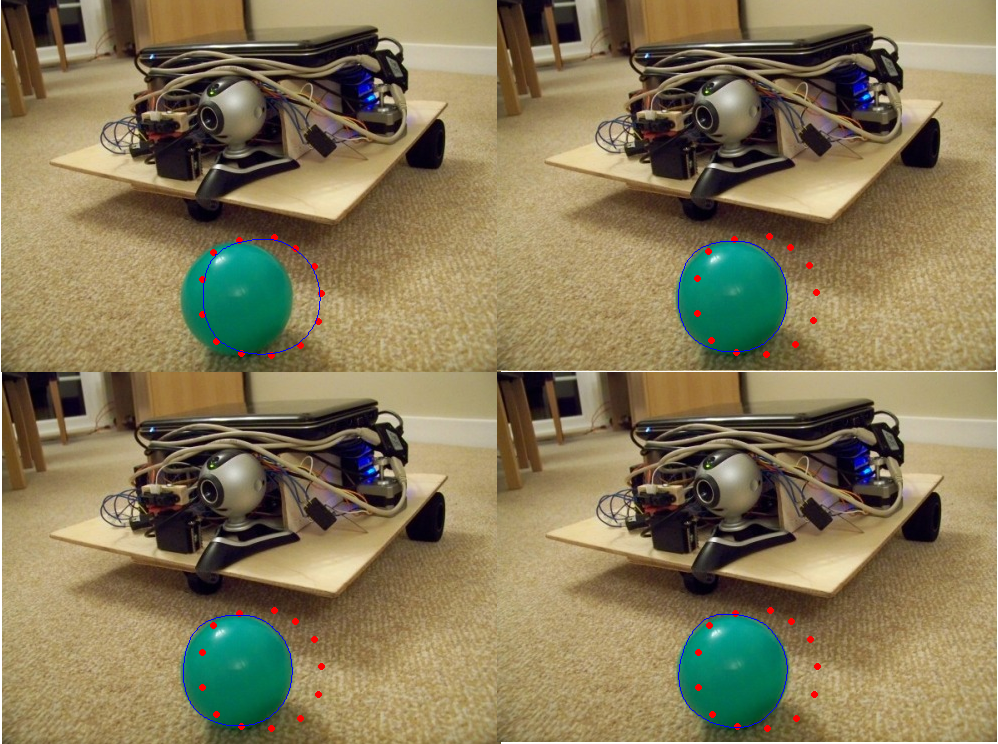
\includegraphics[width=\linewidth]{images/segment1/segment1.png}
  \caption{segmentation result}
  \label{"waiting for reftex-label call..."}
\end{figure}

\begin{figure}[htbp]
  \centering
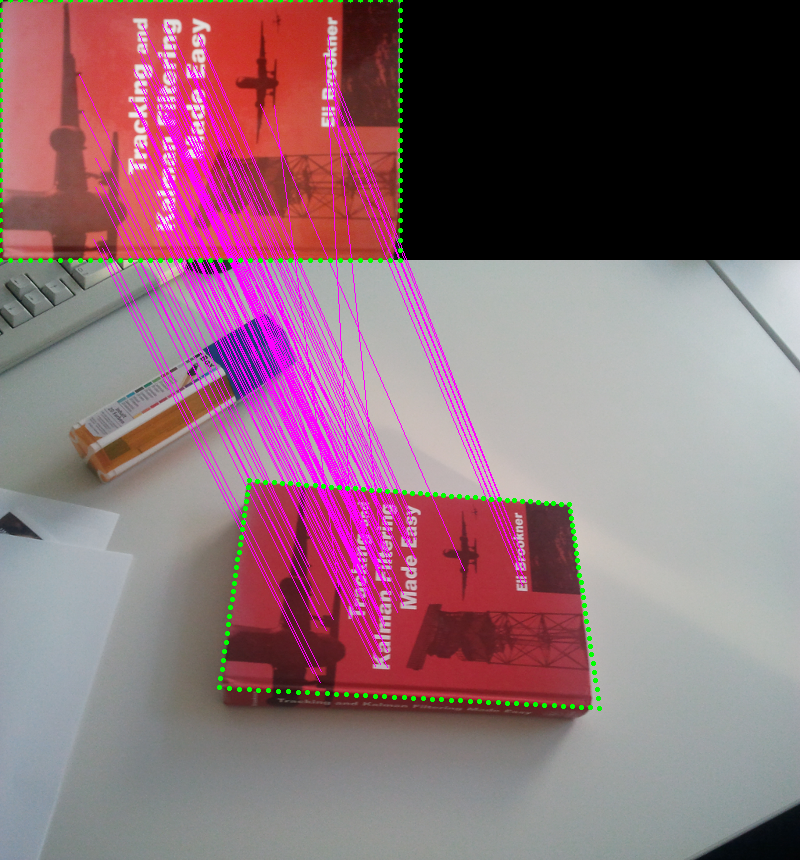
\includegraphics[width=\linewidth]{images/sift.png}
  \caption{sift contour initialization}
  \label{"waiting for reftex-label call..."}
\end{figure}

\begin{figure}[htbp]
  \centering
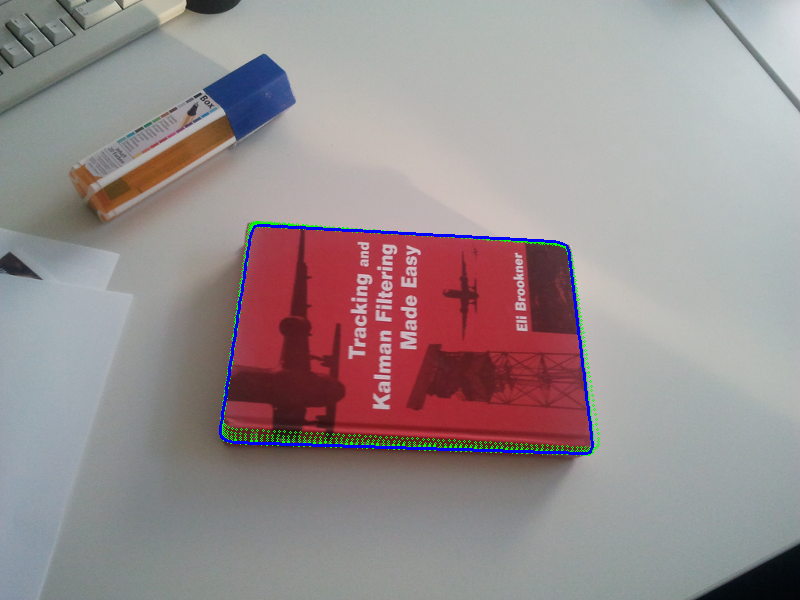
\includegraphics[width=\linewidth]{images/sift_result.png}
  \caption{sift contour initialization}
  \label{"waiting for reftex-label call..."}
\end{figure}
